\documentclass[../experiment.tex]{subfiles}
\graphicspath{{\subfix{../../../images/}}}
\begin{document}
    All The samples were then irradiated with Gamma rays using $^{60}Co$ source first with a
    dose of 5Gy and then 100Gy. After irradiation, 5mg from each sample was then measured and dose response of the 
    samples were recorded utilizing Harshaw TLD reader by heating the sample from $50^{\circ}C$ to $400^{\circ}C$ 
    at a continuous heating rate of $5^{\circ}C/s$. The raw data from Harshaw TLD reader was then plotted using
    Origin software for futher analysis.
    \FloatBarrier\begin{multicols}{2}
        \begin{Figure}
            \centering
            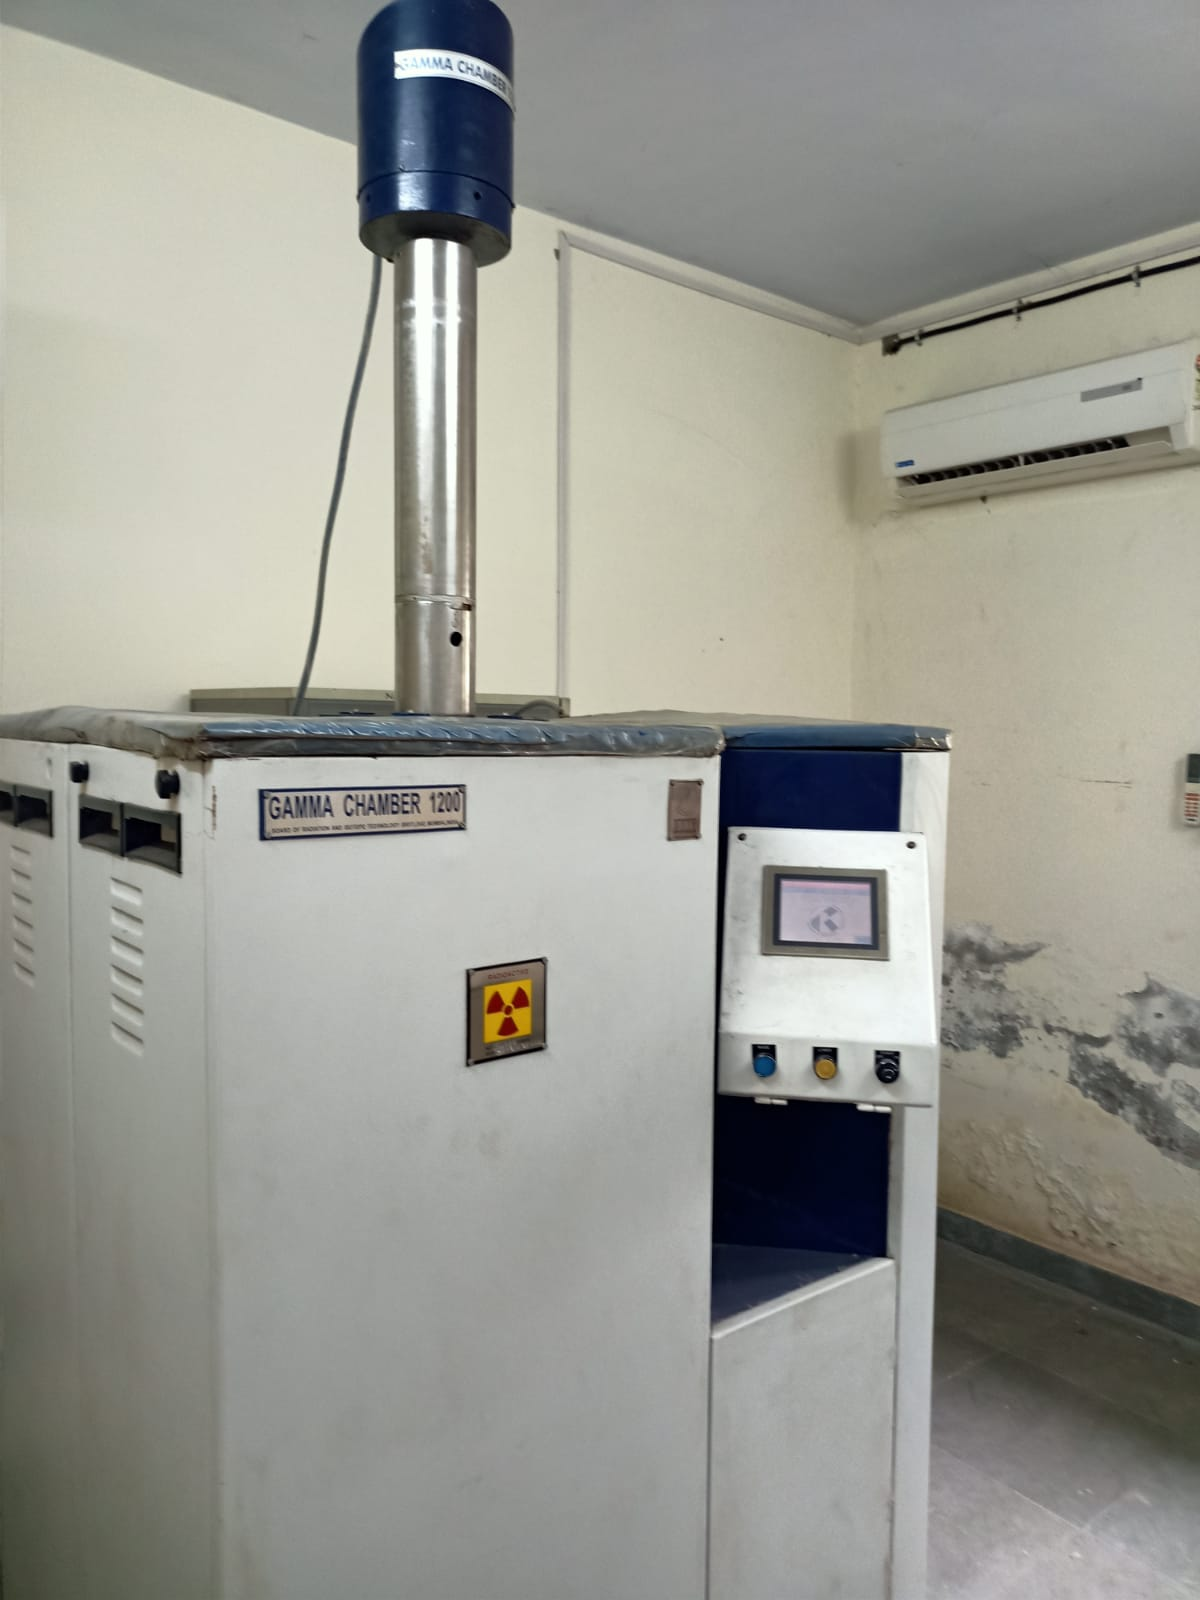
\includegraphics[width=0.6\linewidth]{i1.jpg}
            \captionof{figure}{Gamma ray irradiation chamber at Inter University Accelerator Centre (IUAC), New Delhi
            using $^{60}Co$ source}\label{fig:i1}
        \end{Figure}
        \begin{Figure}
            \centering
            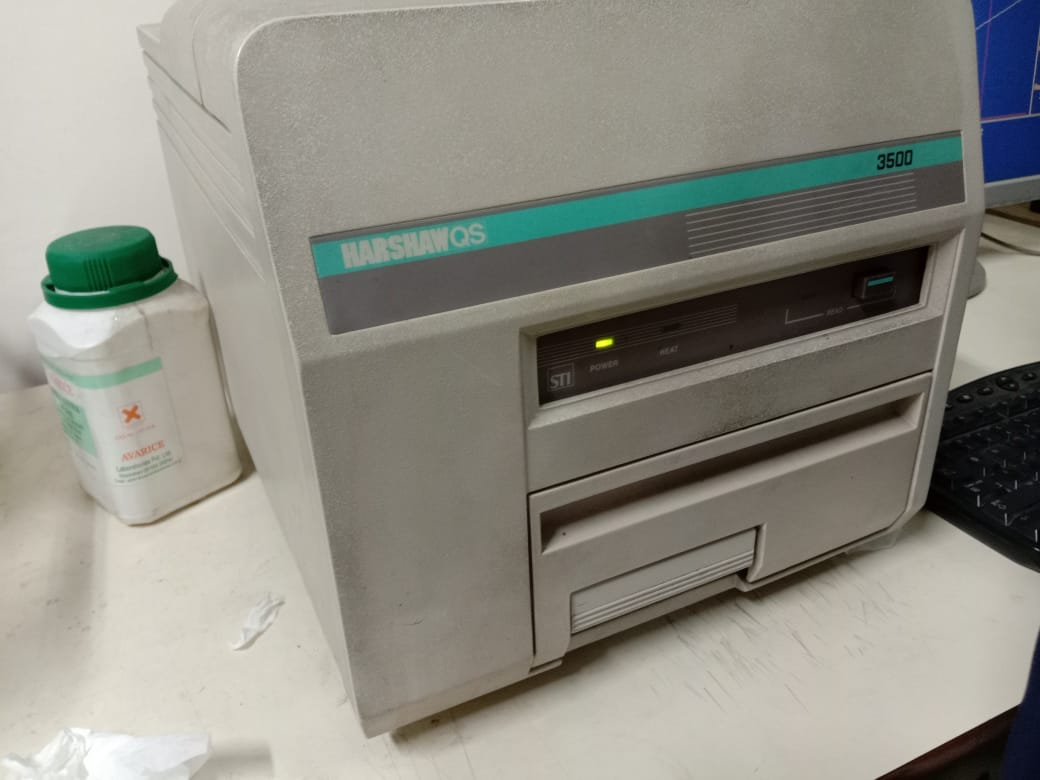
\includegraphics[width=0.6\linewidth]{i2.jpg}
            \captionof{figure}{Harshaw TLD Reader to for measurement of dose response of the samples}\label{fig:i2}
        \end{Figure}
    \end{multicols}
\end{document}